\documentclass{article}
\usepackage[a4paper, total={6in, 10in}]{geometry}
\usepackage[utf8]{inputenc}
\usepackage[english]{babel}
\usepackage{graphicx}
\usepackage{blindtext}
\usepackage{subfiles} % Best loaded last in the preamble
\usepackage[utf8]{inputenc}
\usepackage{verbatim}
\usepackage{fancyhdr}
\usepackage{todonotes}
\usepackage{listings} %For code in appendix
\usepackage[graphicx]{realboxes}
\usepackage{hyperref}
\usepackage[font=small,skip=0pt]{caption}
\setlength{\belowcaptionskip}{-15pt}
\usepackage{comment}
\usepackage{amsmath}
\usepackage{float}
\usepackage{todonotes}
\usepackage{fancyhdr}
\usepackage{lastpage}
\usepackage{enumitem,amssymb}
\newlist{todolist}{itemize}{2}
\setlist[todolist]{label=$\square$}
\usepackage{pifont}
\newcommand{\cmark}{\ding{51}}%
\newcommand{\xmark}{\ding{55}}%
\newcommand{\done}{\rlap{$\square$}{\raisebox{2pt}{\large\hspace{1pt}\cmark}}%
\hspace{-2.5pt}}
\newcommand{\wontfix}{\rlap{$\square$}{\large\hspace{1pt}\xmark}}
\pagestyle{fancy}
\fancyhf{}
\lhead{Course: DevOps, Software Evolution and Software Maintenance, MSc CS (Spring 2021)\\KSDSESM1KU}
\cfoot{\thepage}
\newcommand{\quickcharcount}[1]{%
  \immediate\write18{texcount -1 -sum -merge -char #1.tex > #1-chars.sum}%
  \openin\tmp=#1-chars.sum%
  \read\tmp to \thechar%https://www.overleaf.com/project/5f6c539d2163c50001fdb5f3
  \closein\tmp%
}
\newcommand{\quickwordcount}[1]{%
  \immediate\write18{texcount -1 -sum -merge #1.tex > #1-words.sum}%
  \openin\tmp=#1-words.sum%
  \read\tmp to \theword%
  \closein\tmp%
}

\usepackage[T1]{fontenc}
\usepackage{inconsolata}

\usepackage{color}

\definecolor{pblue}{rgb}{0.13,0.13,1}
\definecolor{pgreen}{rgb}{0,0.5,0}
\definecolor{pred}{rgb}{0.9,0,0}
\definecolor{pgrey}{rgb}{0.46,0.45,0.48}

\usepackage{listings}
\usepackage{xurl}
\title{Exam Report: \\DevOps, Software Evolution and Software Maintenance, MSc CS (Spring 2021)\\
Course code: KSDSESM1KU}
\author{
Frederik Henrik Martini, frem@itu.dk\\
Jesper Falkenberg Henriksen, jefh@itu.dk\\
Jonas Ishøj Nielsen, join@itu.dk \\
Nikolaj Mertz, nime@itu.dk\\
Sif Amalie Rybjerg Kristensen, sikr@itu.dk\\
}
\date{19/05/2021}

\begin{document}

\maketitle

\newpage
{
  \hypersetup{linkcolor=black}
  \tableofcontents
  \clearpage
}



\section{System's perspective} \label{section:System perspective}
\todo{argue for the choice of technologies and decisions for at least all cases for which we asked you to do so in the tasks at the end of each session.}
\subsection{Design} %Jonas

\subsection{Architecture} %Jonas

\subsection{Dependencies (+licencing?) } %Nikolaj %god ide med license her

\subsection{Important interactions of subsystem}

\subsection{Current state of system}
The system is currently has a single known bug regarding the scaling of the system, see section \ref{subsection:scaling}. The tool used for static analysis, \texttt{sonarcloud}, reports the best rating, \textit{A}, on all measures, with 

\begin{itemize}
    \item 0 bugs
    \item 0 code vulnerabilities and 0 security hotspots
    \item 6 hours code debt due to 63 code smells
    \item 0.0\% code duplication and 0 duplicated blocks
\end{itemize}

Out of the 63 code smells only 11 are major, critical or blockers and all 63 has been assessed as issues that can ignored.


\section{Process's perspective} \label{section:Process perspective}
%\todo{Also reflect and describe what was the "DevOps" style of your work. For example, what did you do differently to previous development projects and how did it work?}

\subsection{Interactions and organization of developer team} 
The team used Microsoft Teams for communication with regular meetings every Monday and usually one or two additional "stand up" type meetings throughout the week to check in on progress. Microsoft Teams is also used for links and resources as well as communication regarding individual tasks. Major issues are typically done with everyone present, if they require important decisions, otherwise work is usually done individually or in groups of two or three people - depending on the complexity of the task at hand.

\subsection{CI/CD chain} 
The initial CI/CD was set up using TravisCI, as everyone in the team had encountered it during the lectures. TravisCI was abandoned due to an overwhelming number of issues with files and folders not being added properly, in addition to secret handling being bothersome. We instead settled for using GitHub Actions, which had all the features we wanted (triggers, stages, customizable images and non-local storage of secrets).

The following workflows are set up:
\begin{itemize}
    \item \textbf{Java CI with Maven}: Invoked on all pushes to the repository. It builds the Maven project using \textit{mvn package} and runs all tests, including integration tests on a remote test database. The workflow utilizes caching to ensure that Maven dependencies are not fetched on consecutive runs. 
    \item \textbf{Staging deployment}: Invoked on all pushes to the main branch. This workflow logs into DockerHub, builds and pushes the Minitwit docker image with database secrets. Afterwards it SSHs into the primary Minitwit server and fetches the Minitwit config files, including the docker-compose file. Immediately after, all containers are torn down and rebuild using the newly pushed Minitwit image from DockerHub. Finally, a release is created with new commits linked and the backup server is redeployed similarly. In the downtime of the primary server, the backup server obtains the floating IP and vice versa. 
    \item \textbf{Backup DB}: Once a day a GitHub action SSH into the primary server and creates a database dump with time and date in the name. Created to minimize potential data loss.
    \item \textbf{Build LaTeX document}: When a push to develop occurs, the LaTeX files are fetched from the report folder and a pdf document is built. The LaTeX files are manually fetched from a remote Overleaf repository, as Overleaf facilitates the teams collaborative writing. 
    \item \textbf{SonarCloud}: Official SonarCloud GitHub action that builds and analyzes the Java project using \textit{mvn verify}. 
\end{itemize}
For secret handling we used GitHub's Encrypted secrets. This ensured that no potentially harmful information was exposed in the GitHub Action workflows. Among secrets were DB connection strings, DigitalOcean access tokens, DockerHub credentials and SSH keys together with host information\footnote{\url{https://github.com/DevOps2021-gb/devops2021/wiki/CI-CD-Description:--Github-Actions}}.


\subsection{Organization of repository}
The code is organized using a mono repository setup, having all code and scripts necessary to run the application gathered in a single repository. The team deemed this sufficient as everything located in the repository (apart from local dockerfiles and simulator) is involved in the deployment process and the code-base is small and simple enough that having multiple repositories would only introduce unnecessary complexity

\subsection{Applied branching strategy and development process} 
The main branch is used for the latest release, meaning that the code on this branch matches code found in production. The develop branch facilitated the main development of the project and should always contain a working build. From develop each team member could create feature branches (\texttt{feature/logging} for example) and then merge back into develop once tested and approved. Develop could be subject to hotfixes, which would then be merged into main. The full process can be seen in \underline{\href{https://github.com/DevOps2021-gb/devops2021/blob/main/CONTRIBUTE.md}{CONTRIBUTE.md}}.

The team used GitHub issues to track development progress, labeling them as needed with tags such as \textit{bug}, \textit{documentation}, \textit{feature} and \textit{enhancement}. The status of each issue and the issues to focus on each week was tracked using GitHub's kanban board, having columns \textit{Todo}, \textit{This sprint}, \textit{In progress} and \textit{Done}.

\subsection{Monitoring} 
\label{subsection:monitoring}
Monitoring is set up using Prometheus and Grafana, where Prometheus is used to extract data from the system, and the data is displayed on dashboards in Grafana.

The newest data points are collected and stored using \texttt{MaintenanceService.java}. Each data type is stored in Prometheus library's Gauge or Counter objects, which is registered with a unique name and help description. Data gathered is: the current CPU load, database information and response-time of each endpoint. The data is collected with an interval of 30 seconds. The configuration of Prometheus is found in \texttt{prometheus.yml}\footnote{\url{https://github.com/DevOps2021-gb/devops2021/blob/main/prometheus.yml}}.

On \textit{Grafana} are three dashboards:
\begin{itemize}
    \item \textbf{Minitwit DB info} shows information about the data stored in the database, e.g. the current number of users registered for the application \footnote{\url{http://144.126.244.138:3000/dashboard/db/minitwit-db-info?orgId=1}}.
    \begin{figure}[H]
        \centering
        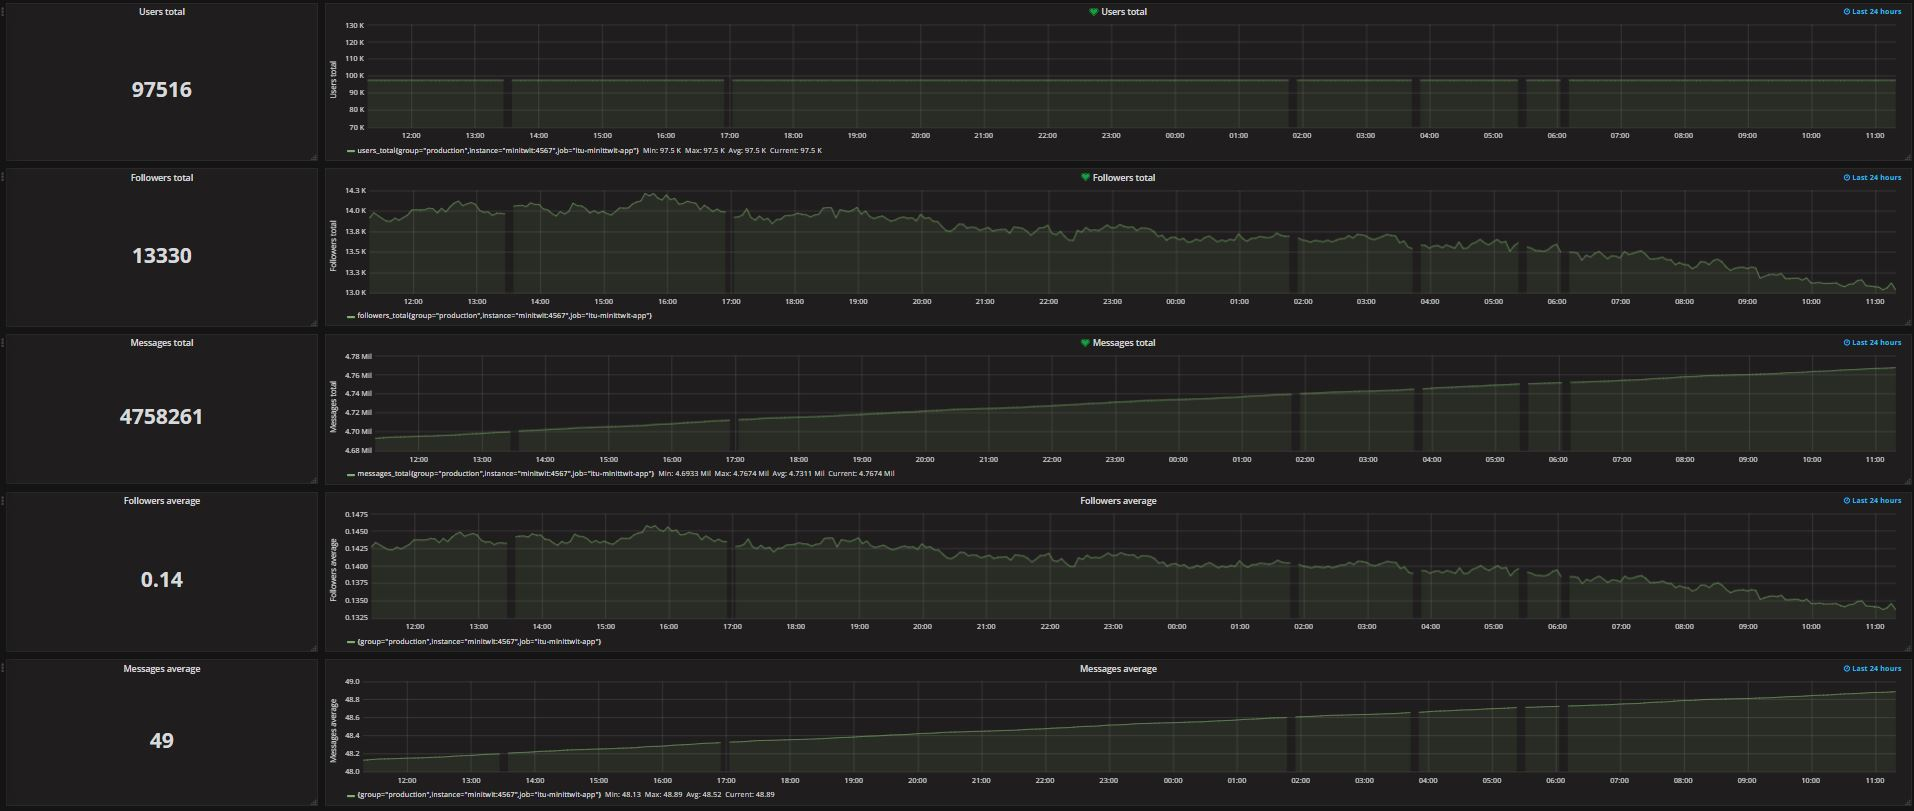
\includegraphics[width=1.0\textwidth]{images/Grafana_minitwit_db.JPG}
        \caption{Grafana dashboard minitwit db}
        \label{fig:grafana_db}
    \end{figure}
    
    \item \textbf{Minitwit request} shows response times for requests to the system.
    \begin{figure}[H]
        \centering
        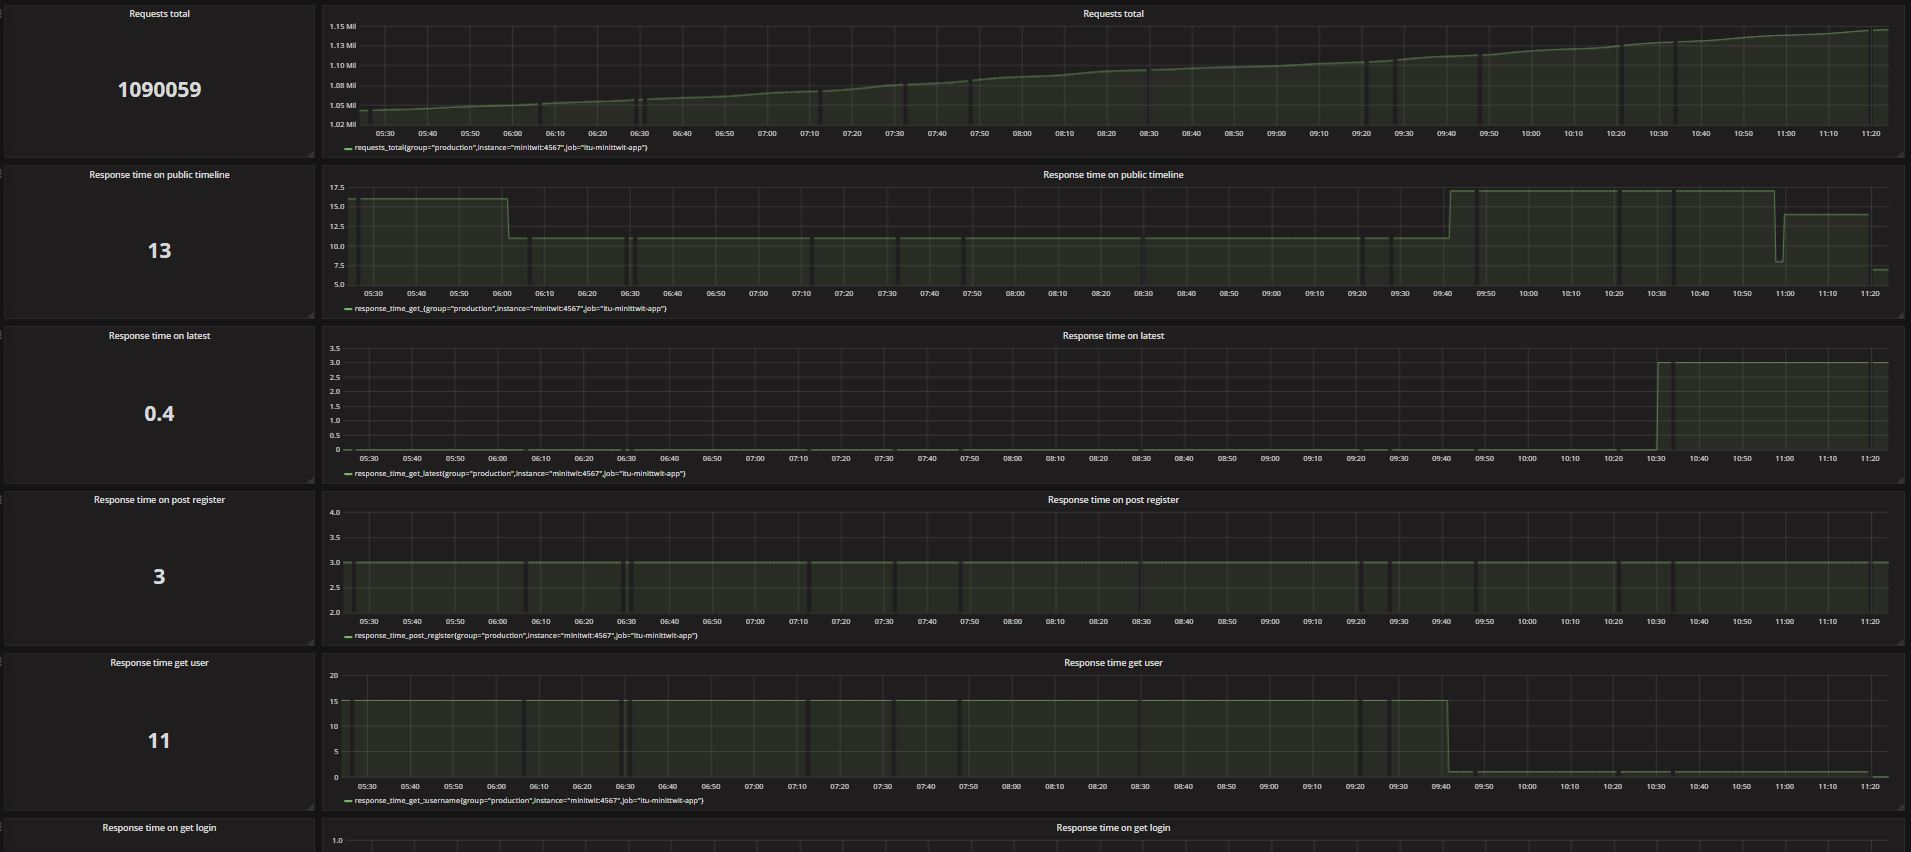
\includegraphics[width=1.0\textwidth]{images/Grafana_minitwit_requests.JPG}
        \caption{Grafana dashboard minitwit requests}
        \label{fig:grafana_requests}
    \end{figure}
    
    \item \textbf{Prometheus Stats} shows the system uptime.
    \begin{figure}[H]
        \centering
        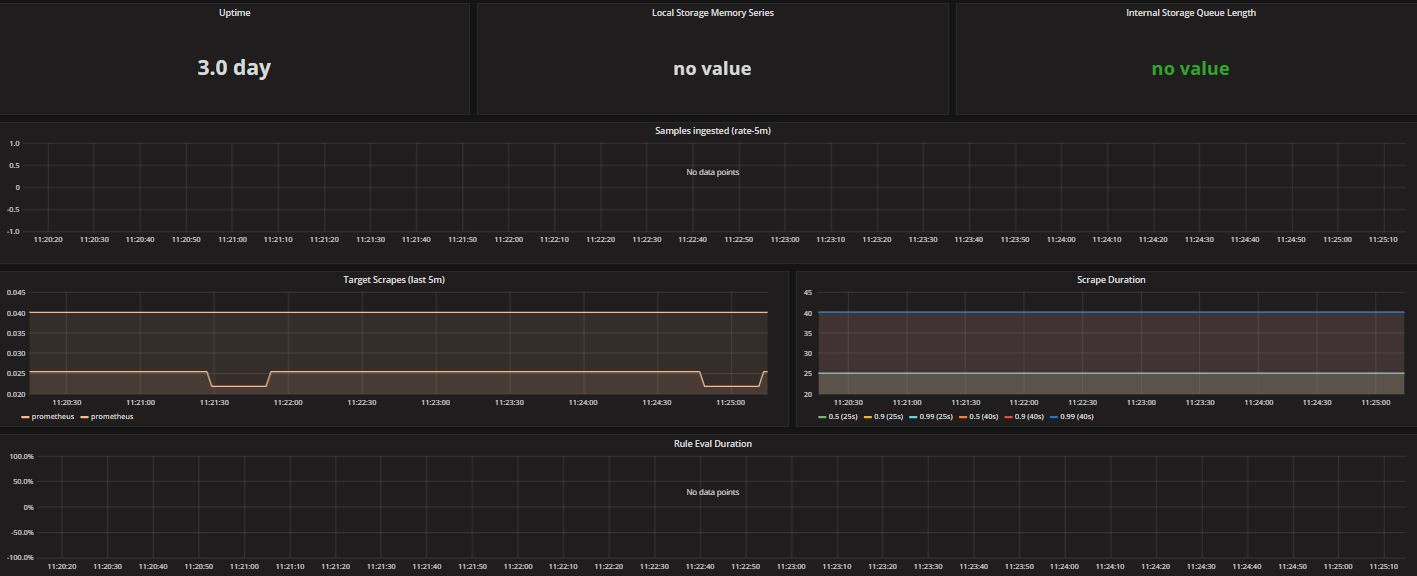
\includegraphics[width=1.0\textwidth]{images/Grafana_prometheous_stats.JPG}
        \caption{Grafana dashboard Prometheus Stats}
        \label{fig:grafana_prometheus}
    \end{figure}
\end{itemize}
The graphs in the dashboards show minimum, maximum and average of the plotted data. The graphs with a heart in the title contains alerts that every 60 seconds check if latest value is below a threshold, indicating that a critical error has occurred. When/if such an alert is triggered Grafana should be setup to email the members of the team, see section \ref{issues-maintenance}.

\subsection{Logging}
\label{subsection:logging}
Logging is set up as an EFK stack. Initially only exceptions were logged but during a test of the logging only one of three introduced bugs was detected, implying that the logging was insufficient. More detailed logging was introduced, now also logging requests and their payloads - except plaintext passwords, which were removed. This change made all three kinds of bugs show up in the log. The description of the experiment can be found in the wiki entry \underline{\href{https://github.com/DevOps2021-gb/devops2021/wiki/Catch-a-Bug-By-Looking-at-the-Logs}{Catch a Bug By Looking at the Logs}}.

Logging is done using Java's Logger object and through our helper-functions each print is extended with a classification/level. The print statements also get a code to easier filter actual warnings rather than messages containing the word 'warning'. The class printing is also added to the message for traceability.

These measures allowed us to create filters for Kibana dashboards such that we could see all messages, all warnings and all of the different kinds of exceptions that could be thrown. A filebeat-elasticsearch index is created once a day for logs and are persistent through Docker volumes. 


\subsection{Security assessment}
In order to assess the security of the system two tasks were undertaken. A risk assessment was conducted and penetration testing was performed. For risk assessment three assets to protect was identified: the web application, the database and the logging. The following potential threats were assessed:
\begin{itemize}
    \item Web application: SQL injection, cross site scripting, DOS, brute forcing login and insufficient logging and monitoring.
    \item Database: SQL injection through web application/API and lost authentication secrets.
    \item Logging: DOS attacks, brute forcing login page.
\end{itemize}

\noindent
A risk analysis table was constructed and 11 scenarios and seven issues were identified and graded. For most of the scenarios actions had already been taken to prevent or mitigate the risks. For a few other scenarios possible actions were identified but not taken as they were deemed unnecessary. The full details of the risks assessment can be found under \underline{\href{https://github.com/DevOps2021-gb/devops2021/wiki/Risk-assesment}{Risk Assessment}}.

For the penetration testing three tools were used: \textit{nmap}, \textit{Metasploit} and \textit{SQL map}. In each case no vulnerabilities were found. In addition to using \textit{SQL map}, cross-site scripting was also tested manually in multiple browsers, by trying to use script-tags in the message input field on the website. In all tested browsers the script tag was not rendered. Lastly, we checked that traces of the tools used showed up in the logging. The full details of the penetration test can be seen in \underline{\href{https://github.com/DevOps2021-gb/devops2021/wiki/Penetration-testing}{Penetration testing}}.

Another group was supposed to perform a white hat attack on the system. Nothing was heard from the group and it must be assumed that they found nothing to report.% or tested another group by mistake.

\subsection{Scaling and load balancing}\label{subsection:scaling} 
The team chose to implement a high-availability setup in terms of a primary and a secondary droplet. First the traditional Heartbeat with Floating IPs on DigitalOcean was implemented\footnote{\url{https://www.digitalocean.com/community/tutorials/how-to-create-a-high-availability-setup-with-heartbeat-and-floating-ips-on-ubuntu-16-04}}. Unfortunately this would only ensure that floating IP were switched to the backup and back again, when the entire machine would go down. We did not find a configuration of Heartbeat that would allow us to listen on a specific port, and switch floating IP's when the Minitwit service was down. We therefore decided to write two shell scripts to gain the sought after functionality. The first script\footnote{\url{https://github.com/DevOps2021-gb/devops2021/tree/main/heartbeat}} continuously runs on the secondary droplet checking the availability of the primary droplet, reassigning the floating-ip to itself should the application on the primary droplet go down. The second script would run on the primary droplet to reassign the floating IP to itself when it has restarted.
\section{Lessons learned perspective} \label{section:Lessons learned perspective}
\subsection{Issues: evolution and refactoring}
Initially, the inherited code was translated to a basic Java application using the Java Spark framework\footnote{\url{https://github.com/DevOps2021-gb/devops2021/issues/152}}. At the time, this code was very bare-bones with all logic and endpoints located in a single file. As time went on, the team refactored the application to make use of a more well structured system architecture (controller-, service-, persistance-layer)\footnote{\url{https://github.com/DevOps2021-gb/devops2021/tree/ae6cd48a06fde2a5c403056b33895b7589cb039d}} eventually adding dependency injection and mock testing\footnote{\url{https://github.com/DevOps2021-gb/devops2021/commit/07914442a09e204f0be2687fe8e5b9bd07799ee4}} to the application. 
During development one of the endpoint's response code was changed which led to a massive increase in errors the simulator reported, which could have been avoided if a fraction of the provided \texttt{minitwit\_simulator.py} file had been a part of the test pipeline.

\subsection{Issues: operation}
\label{issues-operation}
The self-made heartbeat protocol had some issues related to Spark. An issue\footnote{\url{https://github.com/DevOps2021-gb/devops2021/issues/171}} was created trying to remedy this but was never finished, rendering the availability part of the system unstable as the backup would perceive the primary to be down and then reassign the floating-ip to itself exposing a single point of failure. The issue is likely related to Spark's session handling. These scripts can be found in the repository\footnote{\url{https://github.com/DevOps2021-gb/devops2021/tree/main/heartbeat}}

Early on in the project, the database was deployed together with the Minitwit application using Vagrant. Due to SSH key mismanagement, we lost access to our vagrant deployed DigitalOcean Minitwit server containing simulator generated data. Luckily, we were able to reset the root user through Digital Ocean's web terminal functionality. Through this terminal we could add SSH public keys to the \textit{authorized\_keys} file. Finally, we could then SSH into the server and get a database dump. This database dump was based on an outdated model with no ORM, so we had to alter the tables before transferring it to the new remote database server. Only a minor amount of data was lost during the data transfer. To minimize data loss in the future, we created a backup GitHub Action that made a database backup once a day. In addition, SSH keys for the server were backed up in a keystore.

On the 18th of March the webserver crashed due to SSL exceptions. After looking through Docker logs, we narrowed it down to an incompatibility between java-mysql-connector 8.0.15 and Java 11. The solution to this was to update java-mysql-connector 8.0.15 to 8.0.23 \footnote{\url{https://github.com/DevOps2021-gb/devops2021/issues/94}}.

\subsection{Issues: maintenance}
\label{issues-maintenance}
The team never figured out how to make SonarCloud read the test coverage\footnote{\url{https://github.com/DevOps2021-gb/devops2021/issues/140}}, eventually scrapping the idea after spending much time trying to make it work. It should, however, be said that it is able to identify which test functions are proper test functions and that code coverage is obtainable through an IDE like IntelliJ.

Furthermore, the team tried to implement alert notifications on Grafana\footnote{\url{https://github.com/DevOps2021-gb/devops2021/issues/87}} in order to be notified of unexpected data from the monitoring, but this was never successfully implemented.

As the only manual part of the release process, the team had to rename the previous release from 'development release' to the correct tag/version. An issue\footnote{\url{https://github.com/DevOps2021-gb/devops2021/issues/170}} was created in an attempt to automate the entire release process and have an internal counter of the current version, but was never solved.

\subsection{Reflection on DevOps style of work}
The automatic and continuous deployment was very nice to work with since it made it possible for all team members to deploy code without understanding some complicated set of steps to go through. In earlier projects team members have experienced cases where only few group members knew how to deploy.

The idea of having containers, which should enable all members to run the code regardless of tools and dependencies was nice, but the team experienced issues with this resulting in all members still not being able to run the application locally. The issues occurred after adding the EFK stack.

Regarding the way of working together, structuring the repository and branching, this way was not new to any group members but the technique worked well. Some of the techniques group members had used were: making flow visible, limiting work in process, reducing batch/issue sizes and the different ways of eliminating waste in the value stream. In regards to the second way, mobilizing mix of experts and people needing the knowledge has been common practice, and requiring approval near source and experts was common practice. As this is a student project the third ways of creating high-trust culture came naturally.

Adding tests to CI was effective as it removed assumptions and increased resilience of anything committed - and multiple times stopped broken code, which otherwise would have been approved. \\
The logging and maintenance were helpful to provide feedback, allowing us to see the problems as they occurred.


\end{document}